\chapter{Keko}

Keko on tietorakenne, joka pitää yllä alkioiden kokoelmaa
ja tarjoaa seuraavat operaatiot:

\begin{itemize}
\item lisää alkio $x$ joukkoon
\item etsi joukon pienin/suurin alkio
\item poista joukon pienin/suurin alkio
\end{itemize}

Keon toiminta riippuu siitä, onko kyseessä minimikeko
vai maksimikeko.
Minimikeossa voimme etsiä ja poistaa pienimmän alkion,
kun taas maksimikeossa voimme etsiä ja poistaa suurimman alkion.
Meidän täytyy päättää keon luontivaiheessa,
onko keko minimikeko vai maksimikeko.

Tässä luvussa tutustumme binäärikeko-rakenteeseen,
jossa lisäykset ja poistot vievät aikaa $O(\log n)$
ja haku vie aikaa $O(1)$.
Binäärikeko toteutetaan binääripuun avulla,
ja se on tavallisimmin käytetty kekorakenne.
Javan standardikirjaston tietorakenne prioriteettijono
perustuu binäärikekoon.

\section{Binäärikeko}

\emph{Binäärikeko} on binääripuu, jonka jokaisessa solmussa on
yksi kokoelmaan kuuluva alkio.
Puu on rakennettu niin, että sen kaikki tasot alinta
tasoa lukuun ottamatta ovat täynnä solmuja,
eli kaikilla solmuilla on vasen ja oikea lapsi.
Alin taso on puolestaan täytetty niin,
että solmut on sijoitettu mahdollisimman vasemmalle
ylempien solmujen lapsiksi.

Binäärikeon toiminta perustuu siihen,
että jokainen keon solmu täyttää \emph{kekoehdon}.
Minimikeossa kekoehto vaatii, että jokaisen
solmun arvo on suurempi tai yhtä suuri kuin solmun vanhemman arvo.
Maksimikeossa puolestaan jokaisen solmun arvon tulee olla
pienempi tai yhtä suuri kuin solmun vanhemman arvon.
Kekoehdon ansiosta minimikeon juuressa on kokoelman
pienin alkio ja maksimikeon juuressa on kokoelman suurin alkio.

\begin{figure}
\center
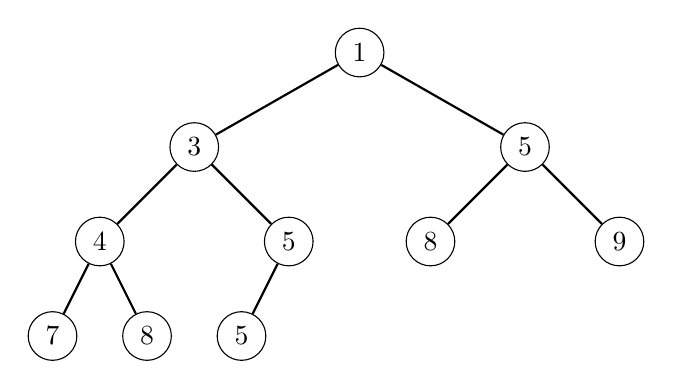
\begin{tikzpicture}[scale=0.6]
\node[draw, circle] (1) at (0,0) {$1$};
\node[draw, circle] (2) at (-3.5,-2) {$3$};
\node[draw, circle] (3) at (3.5,-2) {$5$};
\node[draw, circle] (4) at (-5.5,-4) {$4$};
\node[draw, circle] (5) at (-1.5,-4) {$5$};
\node[draw, circle] (6) at (1.5,-4) {$8$};
\node[draw, circle] (7) at (5.5,-4) {$9$};
\node[draw, circle] (8) at (-6.5,-6) {$7$};
\node[draw, circle] (9) at (-4.5,-6) {$8$};
\node[draw, circle] (10) at (-2.5,-6) {$5$};
\path[draw,thick,-] (1) -- (2);
\path[draw,thick,-] (1) -- (3);
\path[draw,thick,-] (2) -- (4);
\path[draw,thick,-] (2) -- (5);
\path[draw,thick,-] (3) -- (6);
\path[draw,thick,-] (3) -- (7);
\path[draw,thick,-] (4) -- (8);
\path[draw,thick,-] (4) -- (9);
\path[draw,thick,-] (5) -- (10);
\end{tikzpicture}
\caption{Minimikeko, joka vastaa kokoelmaa $[1,3,4,5,5,5,7,8,8,9]$.}
\label{fig:minkek}
\end{figure}


Kuvassa \ref{fig:minkek} on esimerkkinä minimikeko,
johon on tallennettu kymmenen alkiota.
Keon kolme ensimmäistä kerrosta ovat täynnä
ja neljännessä kerroksessa kolme ensimmäistä kohtaa on käytetty.
Keon juurena on kokoelman pienin alkio $1$,
ja kaikki solmut täyttävät kekoehdon.
Huomaa, että sama alkio voi esiintyä keossa useasti,
kuten tässä keossa alkiot $5$ ja $8$.

\subsection{Keon tallentaminen}

Tallennamme binäärikeon \emph{taulukkona},
joka sisältää keon solmujen arvot jär\-jestyksessä
ylhäältä alaspäin ja vasemmalta oikealle.
Tämä tehokas tallennustapa on mahdollinen,
koska keon kaikki tasot ovat täynnä solmuja.
Tallennamme keon taulukkoon kohdasta $1$ alkaen,
koska tämä helpottaa keon operaatioiden toteuttamista.

Esimerkiksi tallennamme kuvan \ref{fig:minkek}
keon taulukkona seuraavasti:

\begin{code}
int[] keko = {0,1,3,5,4,5,8,9,7,8,5};
\end{code}

Huomaa, että taulukon ensimmäinen alkio on $0$,
koska emme käytä kohtaa $0$ keon tallentamiseen.

Tämän tallennustavan etuna on, että voimme laskea
helposti, missä kohdissa keon alkiot ovat taulukossa.
Ensinnäkin keon juuri eli pienin tai suurin alkio
on aina kohdassa $1$.
Lisäksi jos tiedämme, että tietty solmu on kohdassa $k$,
niin tästä seuraa, että

\begin{itemize}
\item solmun vasen lapsi on kohdassa $2k$,
\item solmun oikea lapsi on kohdassa $2k+1$ ja
\item solmun vanhempi on kohdassa $\lfloor k/2 \rfloor$.
\end{itemize}

Esimerkissämme solmu 4
on taulukossa kohdassa $4$,
joten sen lapset ovat kohdissa $8$ ja $9$
ja sen vanhempi on kohdassa $2$.

Käytännössä haluamme yleensä, että pystymme lisäämään kekoon uusia alkioita,
jolloin varaamme suuren taulukon,
jonka alkuosa on keon käytössä ja loppuosassa
on tilaa myöhemmin lisättäville alkioille.

\subsection{Operaatioiden toteutus}

Meidän on helppoa etsiä minimikeon pienin alkio
tai maksimikeon suurin alkio $O(1)$-ajassa,
koska tämä alkio on aina keon juuressa.
Seuraavaksi näemme, kuinka voimme toteuttaa alkion lisäämisen
sekä pienimmän tai suurimman alkion poistamisen $O(\log n)$-ajassa.

\subsubsection{Alkion lisääminen}

Kun lisäämme uuden alkion kekoon, lisäämme sen ensin seuraavaan
vapaana olevaan paikkaan puussa. Jos alimmalla tasolla on tilaa,
lisäämme sen sinne mahdollisimman vasemmalle,
ja muuten aloitamme uuden tason, jossa on toistaiseksi vain lisättävä solmu.
Alkion lisäämisen jälkeen meidän täytyy varmistaa,
että kekoehto säilyy edelleen voimassa.
Tämä tapahtuu siirtämällä alkiota ylöspäin keossa,
kunnes kekoehto tulee voimaan.

\begin{figure}
\center
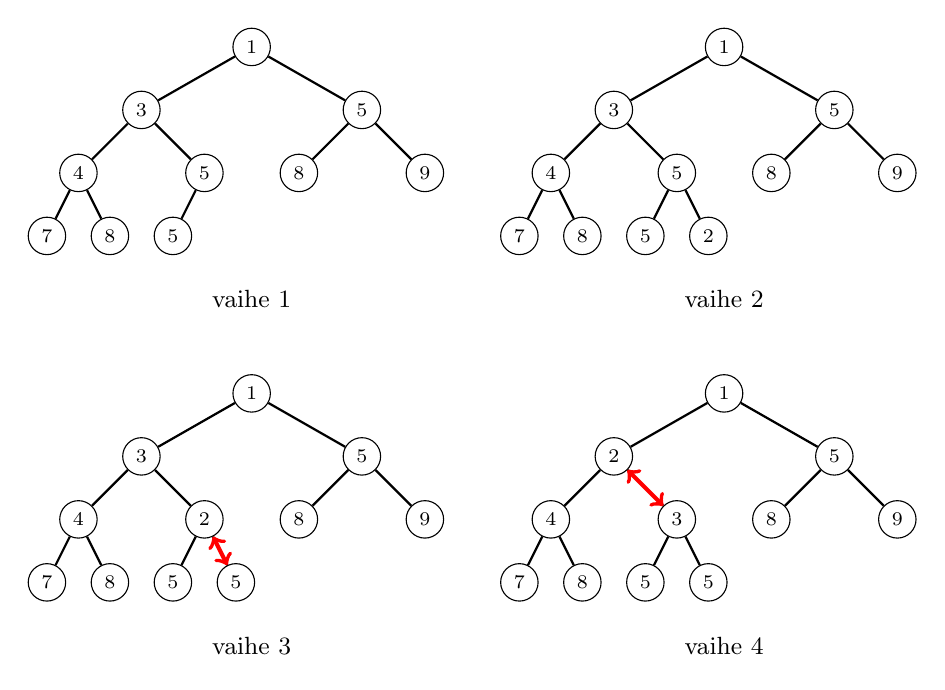
\begin{tikzpicture}[scale=0.4]
\scriptsize
\begin{scope}
\node[draw, circle] (1) at (0,0) {$1$};
\node[draw, circle] (2) at (-3.5,-2) {$3$};
\node[draw, circle] (3) at (3.5,-2) {$5$};
\node[draw, circle] (4) at (-5.5,-4) {$4$};
\node[draw, circle] (5) at (-1.5,-4) {$5$};
\node[draw, circle] (6) at (1.5,-4) {$8$};
\node[draw, circle] (7) at (5.5,-4) {$9$};
\node[draw, circle] (8) at (-6.5,-6) {$7$};
\node[draw, circle] (9) at (-4.5,-6) {$8$};
\node[draw, circle] (10) at (-2.5,-6) {$5$};
\path[draw,thick,-] (1) -- (2);
\path[draw,thick,-] (1) -- (3);
\path[draw,thick,-] (2) -- (4);
\path[draw,thick,-] (2) -- (5);
\path[draw,thick,-] (3) -- (6);
\path[draw,thick,-] (3) -- (7);
\path[draw,thick,-] (4) -- (8);
\path[draw,thick,-] (4) -- (9);
\path[draw,thick,-] (5) -- (10);
\node at (0,-8) {\small vaihe $1$};
\end{scope}
\begin{scope}[xshift=15cm]
\node[draw, circle] (1) at (0,0) {$1$};
\node[draw, circle] (2) at (-3.5,-2) {$3$};
\node[draw, circle] (3) at (3.5,-2) {$5$};
\node[draw, circle] (4) at (-5.5,-4) {$4$};
\node[draw, circle] (5) at (-1.5,-4) {$5$};
\node[draw, circle] (6) at (1.5,-4) {$8$};
\node[draw, circle] (7) at (5.5,-4) {$9$};
\node[draw, circle] (8) at (-6.5,-6) {$7$};
\node[draw, circle] (9) at (-4.5,-6) {$8$};
\node[draw, circle] (10) at (-2.5,-6) {$5$};
\node[draw, circle] (11) at (-0.5,-6) {$2$};
\path[draw,thick,-] (1) -- (2);
\path[draw,thick,-] (1) -- (3);
\path[draw,thick,-] (2) -- (4);
\path[draw,thick,-] (2) -- (5);
\path[draw,thick,-] (3) -- (6);
\path[draw,thick,-] (3) -- (7);
\path[draw,thick,-] (4) -- (8);
\path[draw,thick,-] (4) -- (9);
\path[draw,thick,-] (5) -- (10);
\path[draw,thick,-] (5) -- (11);
\node at (0,-8) {\small vaihe $2$};
\end{scope}
\begin{scope}[yshift=-11cm]
\node[draw, circle] (1) at (0,0) {$1$};
\node[draw, circle] (2) at (-3.5,-2) {$3$};
\node[draw, circle] (3) at (3.5,-2) {$5$};
\node[draw, circle] (4) at (-5.5,-4) {$4$};
\node[draw, circle] (5) at (-1.5,-4) {$2$};
\node[draw, circle] (6) at (1.5,-4) {$8$};
\node[draw, circle] (7) at (5.5,-4) {$9$};
\node[draw, circle] (8) at (-6.5,-6) {$7$};
\node[draw, circle] (9) at (-4.5,-6) {$8$};
\node[draw, circle] (10) at (-2.5,-6) {$5$};
\node[draw, circle] (11) at (-0.5,-6) {$5$};
\path[draw,thick,-] (1) -- (2);
\path[draw,thick,-] (1) -- (3);
\path[draw,thick,-] (2) -- (4);
\path[draw,thick,-] (2) -- (5);
\path[draw,thick,-] (3) -- (6);
\path[draw,thick,-] (3) -- (7);
\path[draw,thick,-] (4) -- (8);
\path[draw,thick,-] (4) -- (9);
\path[draw,thick,-] (5) -- (10);
\path[draw,thick,-] (5) -- (11);
\node at (0,-8) {\small vaihe $3$};
\path[draw,thick,<->,red,line width=1.5pt] (5) -- (11);
\end{scope}
\begin{scope}[yshift=-11cm,xshift=15cm]
\node[draw, circle] (1) at (0,0) {$1$};
\node[draw, circle] (2) at (-3.5,-2) {$2$};
\node[draw, circle] (3) at (3.5,-2) {$5$};
\node[draw, circle] (4) at (-5.5,-4) {$4$};
\node[draw, circle] (5) at (-1.5,-4) {$3$};
\node[draw, circle] (6) at (1.5,-4) {$8$};
\node[draw, circle] (7) at (5.5,-4) {$9$};
\node[draw, circle] (8) at (-6.5,-6) {$7$};
\node[draw, circle] (9) at (-4.5,-6) {$8$};
\node[draw, circle] (10) at (-2.5,-6) {$5$};
\node[draw, circle] (11) at (-0.5,-6) {$5$};
\path[draw,thick,-] (1) -- (2);
\path[draw,thick,-] (1) -- (3);
\path[draw,thick,-] (2) -- (4);
\path[draw,thick,-] (2) -- (5);
\path[draw,thick,-] (3) -- (6);
\path[draw,thick,-] (3) -- (7);
\path[draw,thick,-] (4) -- (8);
\path[draw,thick,-] (4) -- (9);
\path[draw,thick,-] (5) -- (10);
\path[draw,thick,-] (5) -- (11);
\node at (0,-8) {\small vaihe $4$};
\path[draw,thick,<->,red,line width=1.5pt] (2) -- (5);
\end{scope}
\end{tikzpicture}
\caption{Lisäämme alkion 2 kekoon ja nostamme sitä ylöspäin,
kunnes kekoehto tulee jälleen voimaan.}
\label{fig:keklis}
\end{figure}

Kuva \ref{fig:keklis} näyttää, mitä tapahtuu, kun lisäämme
alkion  $2$ esimerkkikekoomme.
Lisäämme alkion ensin seuraavaan vapaaseen kohtaan
keon alimmalla tasolla.
Koska alkio 2 on pienempi kuin sen vanhempi 5,
vaihdamme nämä alkiot keskenään.
Tämän jälkeen alkio 2 on pienempi kuin sen vanhempi 3,
joten vaihdamme myös nämä alkiot keskenään.
Nyt kekoehto on voimassa eikä meidän tarvitse enää
tehdä muutoksia kekoon.

Alkion lisääminen kekoon vie aikaa $O(\log n)$,
koska keossa on $O(\log n)$ tasoa ja kuljemme aina polkua
ylöspäin keon pohjalta huippua kohden,
kunnes olemme löytäneet alkiolle sopivan paikan keosta.

\subsubsection{Alkion poistaminen}

Kun haluamme poistaa keon juuressa olevan alkion,
siirrämme ensin keon viimeisen alkion keon juureksi
ja poistamme sille kuuluneen solmun.
Tämän jälkeen lasketamme juureen nostettua alkiota
alaspäin keossa, kunnes kekoehto tulee jälleen voimaan.
Jos keko on minimikeko, siirrymme alaspäin lapseen,
jossa on pienempi alkio,
ja jos keko on maksimikeko, siirrymme vastaavasti suurempaan alkioon.

\begin{figure}
\center
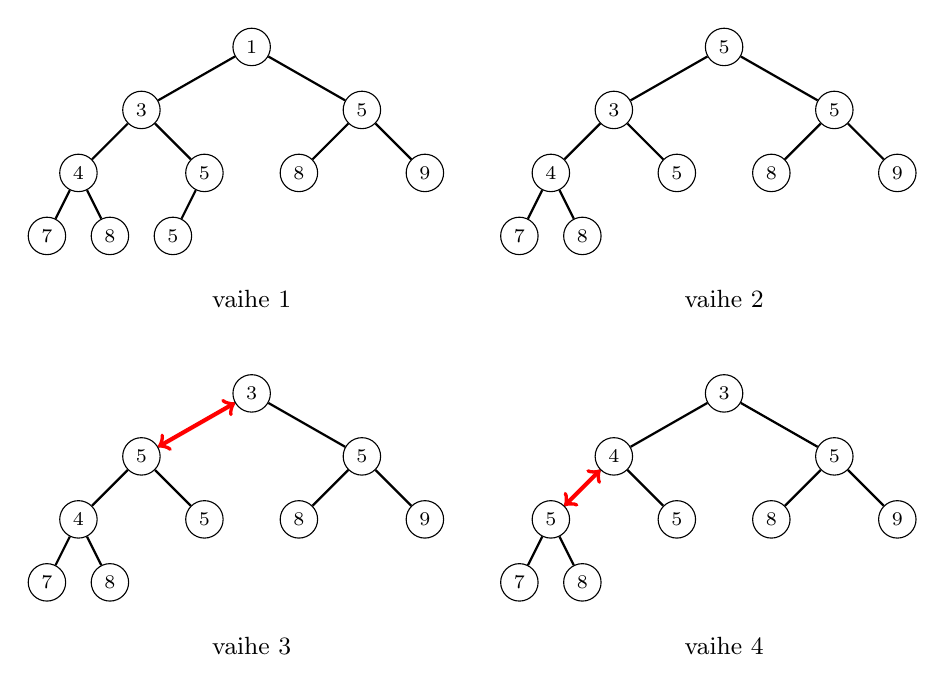
\begin{tikzpicture}[scale=0.4]
\scriptsize
\begin{scope}
\node[draw, circle] (1) at (0,0) {$1$};
\node[draw, circle] (2) at (-3.5,-2) {$3$};
\node[draw, circle] (3) at (3.5,-2) {$5$};
\node[draw, circle] (4) at (-5.5,-4) {$4$};
\node[draw, circle] (5) at (-1.5,-4) {$5$};
\node[draw, circle] (6) at (1.5,-4) {$8$};
\node[draw, circle] (7) at (5.5,-4) {$9$};
\node[draw, circle] (8) at (-6.5,-6) {$7$};
\node[draw, circle] (9) at (-4.5,-6) {$8$};
\node[draw, circle] (10) at (-2.5,-6) {$5$};
\path[draw,thick,-] (1) -- (2);
\path[draw,thick,-] (1) -- (3);
\path[draw,thick,-] (2) -- (4);
\path[draw,thick,-] (2) -- (5);
\path[draw,thick,-] (3) -- (6);
\path[draw,thick,-] (3) -- (7);
\path[draw,thick,-] (4) -- (8);
\path[draw,thick,-] (4) -- (9);
\path[draw,thick,-] (5) -- (10);
\node at (0,-8) {\small vaihe $1$};
\end{scope}
\begin{scope}[xshift=15cm]
\node[draw, circle] (1) at (0,0) {$5$};
\node[draw, circle] (2) at (-3.5,-2) {$3$};
\node[draw, circle] (3) at (3.5,-2) {$5$};
\node[draw, circle] (4) at (-5.5,-4) {$4$};
\node[draw, circle] (5) at (-1.5,-4) {$5$};
\node[draw, circle] (6) at (1.5,-4) {$8$};
\node[draw, circle] (7) at (5.5,-4) {$9$};
\node[draw, circle] (8) at (-6.5,-6) {$7$};
\node[draw, circle] (9) at (-4.5,-6) {$8$};
\path[draw,thick,-] (1) -- (2);
\path[draw,thick,-] (1) -- (3);
\path[draw,thick,-] (2) -- (4);
\path[draw,thick,-] (2) -- (5);
\path[draw,thick,-] (3) -- (6);
\path[draw,thick,-] (3) -- (7);
\path[draw,thick,-] (4) -- (8);
\path[draw,thick,-] (4) -- (9);
\node at (0,-8) {\small vaihe $2$};
\end{scope}
\begin{scope}[yshift=-11cm]
\node[draw, circle] (1) at (0,0) {$3$};
\node[draw, circle] (2) at (-3.5,-2) {$5$};
\node[draw, circle] (3) at (3.5,-2) {$5$};
\node[draw, circle] (4) at (-5.5,-4) {$4$};
\node[draw, circle] (5) at (-1.5,-4) {$5$};
\node[draw, circle] (6) at (1.5,-4) {$8$};
\node[draw, circle] (7) at (5.5,-4) {$9$};
\node[draw, circle] (8) at (-6.5,-6) {$7$};
\node[draw, circle] (9) at (-4.5,-6) {$8$};
\path[draw,thick,-] (1) -- (2);
\path[draw,thick,-] (1) -- (3);
\path[draw,thick,-] (2) -- (4);
\path[draw,thick,-] (2) -- (5);
\path[draw,thick,-] (3) -- (6);
\path[draw,thick,-] (3) -- (7);
\path[draw,thick,-] (4) -- (8);
\path[draw,thick,-] (4) -- (9);
\node at (0,-8) {\small vaihe $3$};
\path[draw,thick,<->,red,line width=1.5pt] (1) -- (2);
\end{scope}
\begin{scope}[yshift=-11cm,xshift=15cm]
\node[draw, circle] (1) at (0,0) {$3$};
\node[draw, circle] (2) at (-3.5,-2) {$4$};
\node[draw, circle] (3) at (3.5,-2) {$5$};
\node[draw, circle] (4) at (-5.5,-4) {$5$};
\node[draw, circle] (5) at (-1.5,-4) {$5$};
\node[draw, circle] (6) at (1.5,-4) {$8$};
\node[draw, circle] (7) at (5.5,-4) {$9$};
\node[draw, circle] (8) at (-6.5,-6) {$7$};
\node[draw, circle] (9) at (-4.5,-6) {$8$};
\path[draw,thick,-] (1) -- (2);
\path[draw,thick,-] (1) -- (3);
\path[draw,thick,-] (2) -- (4);
\path[draw,thick,-] (2) -- (5);
\path[draw,thick,-] (3) -- (6);
\path[draw,thick,-] (3) -- (7);
\path[draw,thick,-] (4) -- (8);
\path[draw,thick,-] (4) -- (9);
\node at (0,-8) {\small vaihe $4$};
\path[draw,thick,<->,red,line width=1.5pt] (2) -- (4);
\end{scope}
\end{tikzpicture}
\caption{Lisäämme alkion 2 kekoon ja nostamme sitä ylöspäin,
kunnes kekoehto tulee jälleen voimaan.}
\label{fig:kekpoi}
\end{figure}

Kuva \ref{fig:kekpoi} näyttää, kuinka poistamme
esimerkkikeostamme pienimmän alkion eli juuressa
olevan alkion 1.
Aluksi korvaamme alkion 1
keon viimeisellä alkiolla 5.
Tämän jälkeen vaihdamme keskenään alkion 5
ja sen vasemman lapsen alkion 3,
ja sitten vielä alkion 5 ja sen vasemman lapsen alkion 4.
Tämän jälkeen kekoehto on voimassa ja olemme onnistuneet
poistamaan pienimmän alkion keosta.

Alkion poistaminen keosta vie aikaa $O(\log n)$,
koska keossa on $O(\log n)$ tasoa ja kuljemme polkua
alaspäin keon huipulta pohjaa kohden.

\section{Prioriteettijono}

Monissa ohjelmointikielissä kekoa vastaava tietorakenne
tunnetaan nimellä \emph{prioriteettijono}.
Näin on myös Javassa, jonka standardikirjastoon 
kuuluu tietorakenne \texttt{PriorityQueue}.
Se on binäärikekoon perustuva tietorakenne,
joka toteuttaa oletuksena minimikeon.

Seuraava koodi esittelee Javan prioriteettijonon toimintaa.
Metodi \texttt{add} lisää alkion jonoon,
metodi \texttt{peek} hakee pienimmän alkion
ja metodi \texttt{poll} hakee ja poistaa pienimmän alkion.

\begin{code}
PriorityQueue<Integer> jono = new PriorityQueue<>();
jono.add(5);
jono.add(3);
jono.add(8);
jono.add(7);
System.out.println(jono.peek()); // 3
System.out.println(jono.poll()); // 3
System.out.println(jono.poll()); // 5
\end{code}

Jos haluamme luoda prioriteettijonon, joka onkin
maksimikeko, voimme tehdä sen seuraavaan tapaan:

\begin{code}
PriorityQueue<Integer> jono =
    new PriorityQueue<>(10,Collections.reverseOrder());
\end{code}

Tässä tilanteessa meidän täytyy antaa konstruktorille kaksi tietoa:
keolle alussa muistista varattava tila (tässä 10)
sekä alkioiden järjestämistapa (tässä käänteinen järjestys).
Java varaa keolle tarvittaessa myöhemmin uuden suuremman muistialueen,
joten tämä määrittely ei tarkoita, että keossa voisi olla enintään 10 alkiota.

Jos haluamme tallentaa prioriteettijonoon omia olioitamme,
meidän tulee toteuttaa luokkaan metodi \texttt{compareTo} ja
merkitä, että luokka toteuttaa rajapinnan \texttt{Comparable}.

\section{Tehokkuusvertailu}

Mitä hyötyä keosta oikeastaan on?
Meillähän on olemassa jo binäärihakupuu,
jonka avulla voimme toteuttaa kaikki keon operaatiot
ja \emph{enemmänkin}.
Keossa voimme hakea ja poistaa vain pienimmän tai suurimman alkion,
mutta binäärihakupuussa voimme käsitellä myös muita alkioita.

Keon etuna on, että siinä on tehokkaan taulukkototeutuksen
ansiosta pienemmät \emph{vakiokertoimet} kuin binäärihakupuussa.
Jos meille riittää, että voimme hakea ja poistaa
vain pienimmän tai suurimman alkion, voi siis olla hyvä
ratkaisu käyttää kekoa binäärihakupuun sijasta.
Mutta kuinka suuria erot ovat käytännössä?

Teemme seuraavaksi testin, jossa vertailemme keskenään
Javan rakenteita
\texttt{PriorityQueue} ja \texttt{TreeSet}.
Testissä meillä on taulukko,
jossa on satunnaisessa järjestyksessä luvut $1,2,\dots,n$.
Lisäämme ensin taulukon $n/2$ ensimmäistä lukua kokoelmaan.
Tämän jälkeen käymme läpi loput $n/2$ lukua,
ja jokaisen luvun kohdalla lisäämme sen kokoelmaan ja
poistamme kokoelman pienimmän luvun.
Laskemme lisäksi samalla summaa poistetuista luvuista.
Käytämme testissä seuraavia koodeja:

\begin{code}
PriorityQueue<Integer> jono = new PriorityQueue<>();
for (int i = 0; i < n/2; i++) {
    jono.add(luvut[i]);
}
long summa = 0;
for (int i = n/2; i < n; i++) {
    jono.add(luvut[i]);
    summa += jono.poll();
}
System.out.println(summa);
\end{code}

\begin{code}
TreeSet<Integer> joukko = new TreeSet<>();
for (int i = 0; i < n/2; i++) {
    joukko.add(luvut[i]);
}
long summa = 0;
for (int i = n/2; i < n; i++) {
    joukko.add(luvut[i]);
    summa += jono.pollFirst();
}
System.out.println(summa);
\end{code}

Taulukko \ref{tab:kekver} sisältää vertailun tulokset.
Tämän testin perusteella näyttää siltä,
että keon käyttämiseestä on todellista hyötyä,
koska \texttt{PriorityQueue} toimii 2–3
kertaa nopeammin kuin \texttt{TreeSet}.

\begin{table}
\center
\begin{tabular}{rrrr}
taulukon koko $n$ & \texttt{PriorityQueue} & \texttt{TreeSet} \\
\hline
$10^6$ & 0.29 s & 0.78 s \\
$2 \cdot 10^6$ & 0.71 s & 1.50 s \\
$4 \cdot 10^6$ & 1.56 s & 3.72 s \\
$8 \cdot 10^6$ & 3.68 s & 9.43 s \\
\end{tabular}
\caption{Algoritmien suoritusaikojen vertailu.}
\label{tab:kekver}
\end{table}

\section{Lisää keosta}

\subsection{Tehokas luonti}

Suoraviivainen tapa luoda $n$ alkiota sisältävä keko
on lisätä jokainen alkio erikseen kekoon $O(\log n)$-ajassa.
Tällä tavalla saamme rakennettua keon $O(n \log n)$-ajassa.
Osoittautuu kuitenkin, että keon luominen taulukon pohjalta
on mahdollista myös $O(n)$-ajassa.

Ideana on käydä läpi keon solmut lopusta alkuun ja
jokaisen solmun kohdalla varmistaa,
että siitä solmusta alkava alipuu toteuttaa kekoehdon
laskettamalla solmun juuressa olevaa arvoa alaspäin.
Kun olemme lopulta käsitelleet kaikki solmut juureen asti,
koko taulukko toteuttaa kekoehdon.

Miksi sitten tämä vie aikaa vain $O(n)$?
Oletetaan, että keossa on $h$ kerrosta ja kaikki
kerrokset ovat täynnä solmuja, eli siinä on $n=2^h-1$ solmua.
Laskemme jokaiselle kerrokselle, montako arvoa laskeutuu
enintään jostakin tämän kerroksen solmusta alaspäin. Tästä saamme:

\begin{itemize}
\item Kerroksesta 1 kerrokseen 2 laskeutuu enintään 1 arvo.
\item Kerroksesta 2 kerrokseen 3 laskeutuu enintään $1+2$ arvoa.
\item Kerroksesta 3 kerrokseen 4 laskeutuu enintään $1+2+4$ arvoa.
\item Jne.
\end{itemize}

Yleisemmin kerroksesta $k$ kerrokseen $k+1$ laskeutuu
enintään $1+2+\dots+2^{k-1} = 2^k-1$ arvoa.
Koska kerroksia on $h$ ja viimeisestä kerroksesta ei voi laskeutua alaspäin,
kokonaistyömäärä on enintään
\[(2^1-1)+(2^2-1)+\dots+(2^{h-1}-1)=2^h-h \le n,\]
joten aikaa kuluu vain $O(n)$.

\subsection{Kekojärjestäminen}

